% `template.tex', a bare-bones example employing the AIAA class.
%
% For a more advanced example that makes use of several third-party
% LaTeX packages, see `advanced_example.tex', but please read the
% Known Problems section of the users manual first.
%
% Typical processing for PostScript (PS) output:
%
%  latex template
%  latex template   (repeat as needed to resolve references)
%
%  xdvi template    (onscreen draft display)
%  dvips template   (postscript)
%  gv template.ps   (onscreen display)
%  lpr template.ps  (hardcopy)
%
% With the above, only Encapsulated PostScript (EPS) images can be used.
%
% Typical processing for Portable Document Format (PDF) output:
%
%  pdflatex template
%  pdflatex template      (repeat as needed to resolve references)
%
%  acroread template.pdf  (onscreen display)
%
% If you have EPS figures, you will need to use the epstopdf script
% to convert them to PDF because PDF is a limmited subset of EPS.
% pdflatex accepts a variety of other image formats such as JPG, TIF,
% PNG, and so forth -- check the documentation for your version.
%
% If you do *not* specify suffixes when using the graphicx package's
% \includegraphics command, latex and pdflatex will automatically select
% the appropriate figure format from those available.  This allows you
% to produce PS and PDF output from the same LaTeX source file.
%
% To generate a large format (e.g., 11"x17") PostScript copy for editing
% purposes, use
%
%  dvips -x 1467 -O -0.65in,0.85in -t tabloid template
%
% For further details and support, read the Users Manual, aiaa.pdf.


% Try to reduce the number of latex support calls from people who
% don't read the included documentation.
%
\typeout{}\typeout{If latex fails to find aiaa-tc, read the README file!}
%


\documentclass[]{aiaa-tc}% insert '[draft]' option to show overfull boxes
\usepackage{float}
 \title{Stability and Control Considerations in STOVL Aircraft Design}

 \author{
  K. Volle\footnote{Graduate Research Student, Robotics}%
    %\thanks{Job Title, Department, Address, and AIAA Member Grade.}
  \ and J. Rogers\footnote{Associate Professor, Mechanical Engineering}\\%\thanksibid{1}\\
  {\normalsize\itshape
   Georgia Institute of Technology, Atlanta, Ga, 30318}\\
 % \and
 % Third C. Author%
  % \thanks{Job Title, Department, Address, and AIAA Member Grade.}\\
  %{\normalsize\itshape
 % Business or Academic Affiliation, City, Province, Zipcode, Country}
 }

 % Data used by 'handcarry' option if invoked
 \AIAApapernumber{YEAR-NUMBER}
 \AIAAconference{Conference Name, Date, and Location}
 \AIAAcopyright{\AIAAcopyrightD{YEAR}}

 % Define commands to assure consistent treatment throughout document
 \newcommand{\eqnref}[1]{(\ref{#1})}
 \newcommand{\class}[1]{\texttt{#1}}
 \newcommand{\package}[1]{\texttt{#1}}
 \newcommand{\file}[1]{\texttt{#1}}
 \newcommand{\BibTeX}{\textsc{Bib}\TeX}

\begin{document}

\maketitle

\begin{abstract}
There is an increasing demand for unmanned aerial vehicles (UAVs)that are capable of performing multiple or hybrid mission profiles.  The Pterodactyl UAV is designed to transition between multiple flight modes so as to make it more suitable to a variety of mission profiles. The Pterodactyl incorporates morphing wing methods into a tailsitter concept. resulting in a vehicle with a wide range of applications. The robustness of the vehicle configuration and controller design is examined by looking at the effects of the vehicle geometry and by simulating the vehicle orienting itself in response to initial perturbations.
\end{abstract}

\section*{Nomenclature}



\begin{tabbing}
  XXX \= \kill% this line sets tab stop
\centering
  $ \phi_{L} $ \> Left wing cant angle \\
  $ \phi_{R} $ \> Right wing cant angle \\
  $ \psi $ \> Fold line angle \\
  $ H $ \> Distance along leading edge from sagittal plane to fold line  \\
  $ P $ \> Distance along leading edge from fold line to propulsor location \\

 \end{tabbing}
\section{Introduction}

The Pterodactyl unmanned aerial system concept is a tailsitter \cite{Forshaw:2012} vehicle that autonomously takes advantage of its morphing capability to gain the ability to fit multiple applications. The ultimate goal is a vehicle that can be deployed, operated and recovered entirely from a small, mobile platform such as a truck bed.
DARPA perfectly expressed the importance of developing systems such as this in their program call for the UAVForge project, saying that "Persistent, beyond-line-of-sight, soldier-portable perch and stare intelligence, surveillance and reconnaissance (ISR) is a significant mission area of interest that shows promising capability\footnote{\textit{http://www.darpa.mil}} \ldots  "

The inspiration for the Pterodactyl can be found in nature. Birds, for example, change their configuration when performing aerial maneuvers including diving, loitering, or swooping to land. The ability to make large scale changes to their aerodynamic properties is vital to achieving the versatility that birds exhibit. Morphing in this context is any substantial change in the geometry of the vehicle that alters its aerodynamic properties.\cite{Barbarino:2011} Control surface deflections are not themselves sufficient to be considered morphing, but may be utilized in one or more of the vehicle modes as well as in the transitions between modes.\cite{Wickenheiser:2008} Examples of morphing include, but are not limited to: alterations in span, sweep and/or chord of the wings, wing twist, wing bending, and airfoil adjustment.

Unlike many convertiplane designs, the Pterodactyl will rotate the entire vehicle during transition. This will simplify the design and control without losing the abilities for both vertical and horizontal flight.\cite{Stone:2008} Despite numerous efforts to improve the design and control of tailsitter aircraft, the development of a vehicle that effectively combines the forward and vertical flighty capabilities remains an open question.\cite{Escareno:2007}\cite{Matsumoto:2010}

This paper discusses vehicle geometry for controllability, and design of an attitude controller for the
Pterodactyl UAV in the hover condition. Simulation of the forward flight and transition processes are left to future studies.


\section{Design Overview}
A typical usage case for the Pterodactyl begins with the vehicle being launched from a rail-type device that is no longer than 6 feet. Once airborne, the Pterodactyl acts as a tailless fixed-wing craft and autonomously executes its mission with flight speeds between 35-100 knots. Upon completing its mission and returning to the launch platform, the vehicle performs a rapid climb maneuver in which it transitions to vertical flight. At this point the wings will fold about hinges partway down each wing to form a roughly triangular configuration with three non-parallel thrust vectors. The two primary modes are illustrated in Figures ~\ref{fig:forward} and ~\ref{fig:hover}. This configuration has several advantages, the most important of which are listed below.
\newline
\newline
\textbullet \hspace{1 pt} The three linearly independent thrust vectors give complete control over vehicle orientation.
\newline
\textbullet \hspace{1 pt} The compact and convex form factor exposes less area to the wind, improving gust-rejection.
\newline
\textbullet \hspace{1 pt} The wings will fold about the payload which will help to protect sensitive electronics.
\newline
\textbullet \hspace{1 pt} Much less space is required for landing.
\begin{figure}[ht]
\centering
\begin{minipage}[b]{0.45\linewidth}
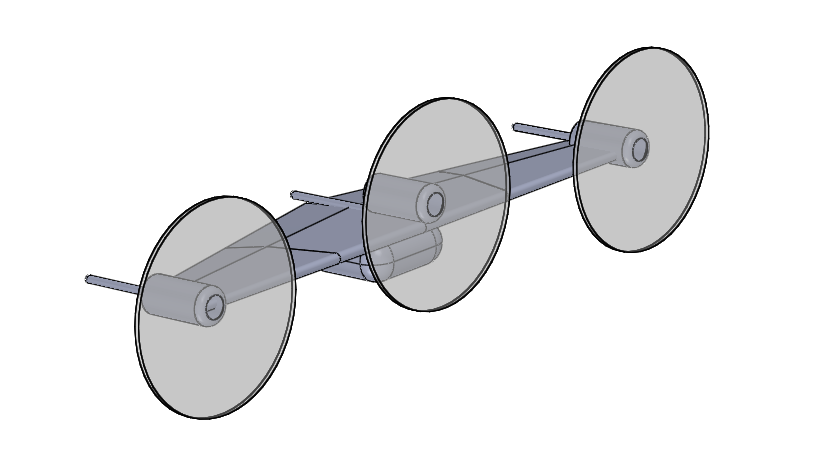
\includegraphics[width=1\textwidth]{pterodactylForward}
\caption{Forward Flight Configuration}
\label{fig:forward}
\end{minipage}
\quad
\begin{minipage}[b]{0.45\linewidth}
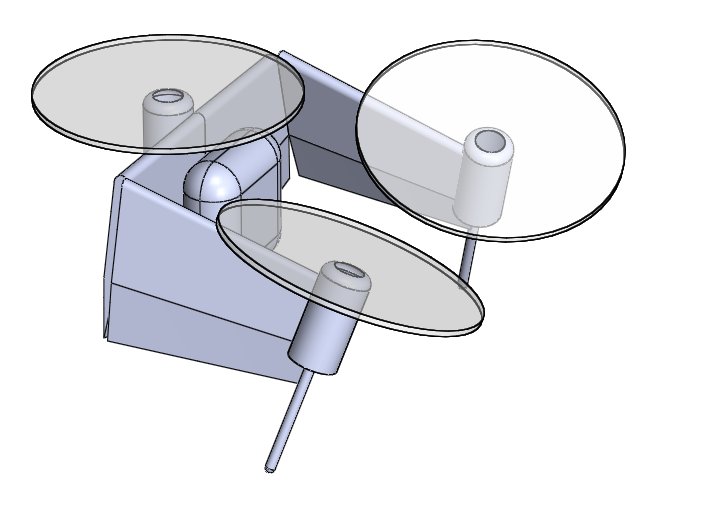
\includegraphics[width=1\textwidth]{pterodactylHover}
\caption{Hover Configuration}
\label{fig:hover}
\end{minipage}
\end{figure}

It is plain to see from the above consideration that a successful design is heavily dependent on the vehicle's geometry.  For this paper the hinge line angle ($\psi$) is assumed to be the same for each side, though this constraint isn't required. We can draw conclusions about the parameter selection without relaxing this constraint by taking advantage of the symmetry of the vehicle. The geometric parameters under consideration are described in Table ~\ref{fig:geometry}.
\begin{figure}
\begin{center}
\caption{Representative Geometry Parameters}
	\begin{tabular}{| c | c |}
	\hline
	Parameter & Value \\ \hline \hline
 	 $ \psi $  & $15^{\circ}$ \\ \hline
 	 $ \phi_{L} $  & $120^{\circ}$ \\ \hline
 	 $ \phi_{R} $  & $110^{\circ}$ \\ \hline
 	 $ H $ & 1.75 ft\\ \hline
 	 $ P $ & 0.75 ft\\ \hline
 	 
	\end{tabular}
	\label{fig:geometry}
	\end{center}
\end{figure}
To evaluate a given configuration, we define a matrix A that represents a linear transformation from thrusts to moments about the center of mass of the vehicle. It is important to note that control of the vehicle in hover comes from differential thrust of the three propulsors since the propeller blades will have a fixed pitch and the orientations of the thrust vectors relative to the propulsor support structures are fixed.
The column vectors of A corresponding to each propulsor are the cross product of the position of that propulsor relative to the center of mass and the orientation of the thrust vector in body coordinates. The closed form of the position vector is as follows:
\[ \left( \begin{array}{ccc}
comY + P(cos(\psi)sin(\phi_{R})) \\
H– comY +P(cos(\phi_{R})cos^{2}(\psi) + sin^{2}(\psi)) \\
comZP(cos(\psi)sin(\psi) – cos(\phi_{R})cos(\psi)sin(\psi)) \end{array} \right) \]
The closed form of the orientation vector is as follows:
\[ \left( \begin{array}{ccc}
sin(\psi) sin(\phi_{R}) \\
sin(\psi) cos(\psi) cos(\phi_{R}) – sin(\psi) cos(\psi)\\
-cos^{2}(\psi) - cos(\phi_{R})sin^{2}(\psi) \end{array} \right)
 \]
The sums of the absolute values of the elements of the component row vectors and the condition number are the most useful properties of this matrix for evaluating a given configuration. The first property is a metric of the magnitude of the moments that are achievable from the set of available forces. The condition number is a metric of the invertability of a matrix. This is important because calculating commanded thrusts from the required moments requires taking the inverse of A.

The geometry is also used to numerically approximate the principal moments of inertia of the vehicle. At this stage of vehicle design, however, this calculation requires too many assumptions about the mass distribution of the vehicle to be of use quantitatively. Qualitatively, one can see that the ratio of achievable moment about a body axis to the moment of inertia about that same axis should be maximized so as to improve the response of the vehicle.

\section{Controller Design}

The simulation used a proportional-derivative controller to return to the desired orientation from an initial perturbed orientation. The orientation here is expressed as Tait-Bryan angles, specifically the roll-pitch-yaw notation. The angles are denoted a s $\phi$, $\theta$, $\psi$ respectively. Figure ~\ref{fig:control} shows the basic block diagram governing this controller. It is important to note that since the three rotations are treated independently and in parallel the values of $K_{p} $ and $K_{d}$ can be set individually for each axis. This controller was shown to be stable in simulation provided the gains are set such that the required thrusts do not exceed the vehicle’s capabilities.
\begin{figure}[H]
\caption{Block diagram for attitude controller.}
\center
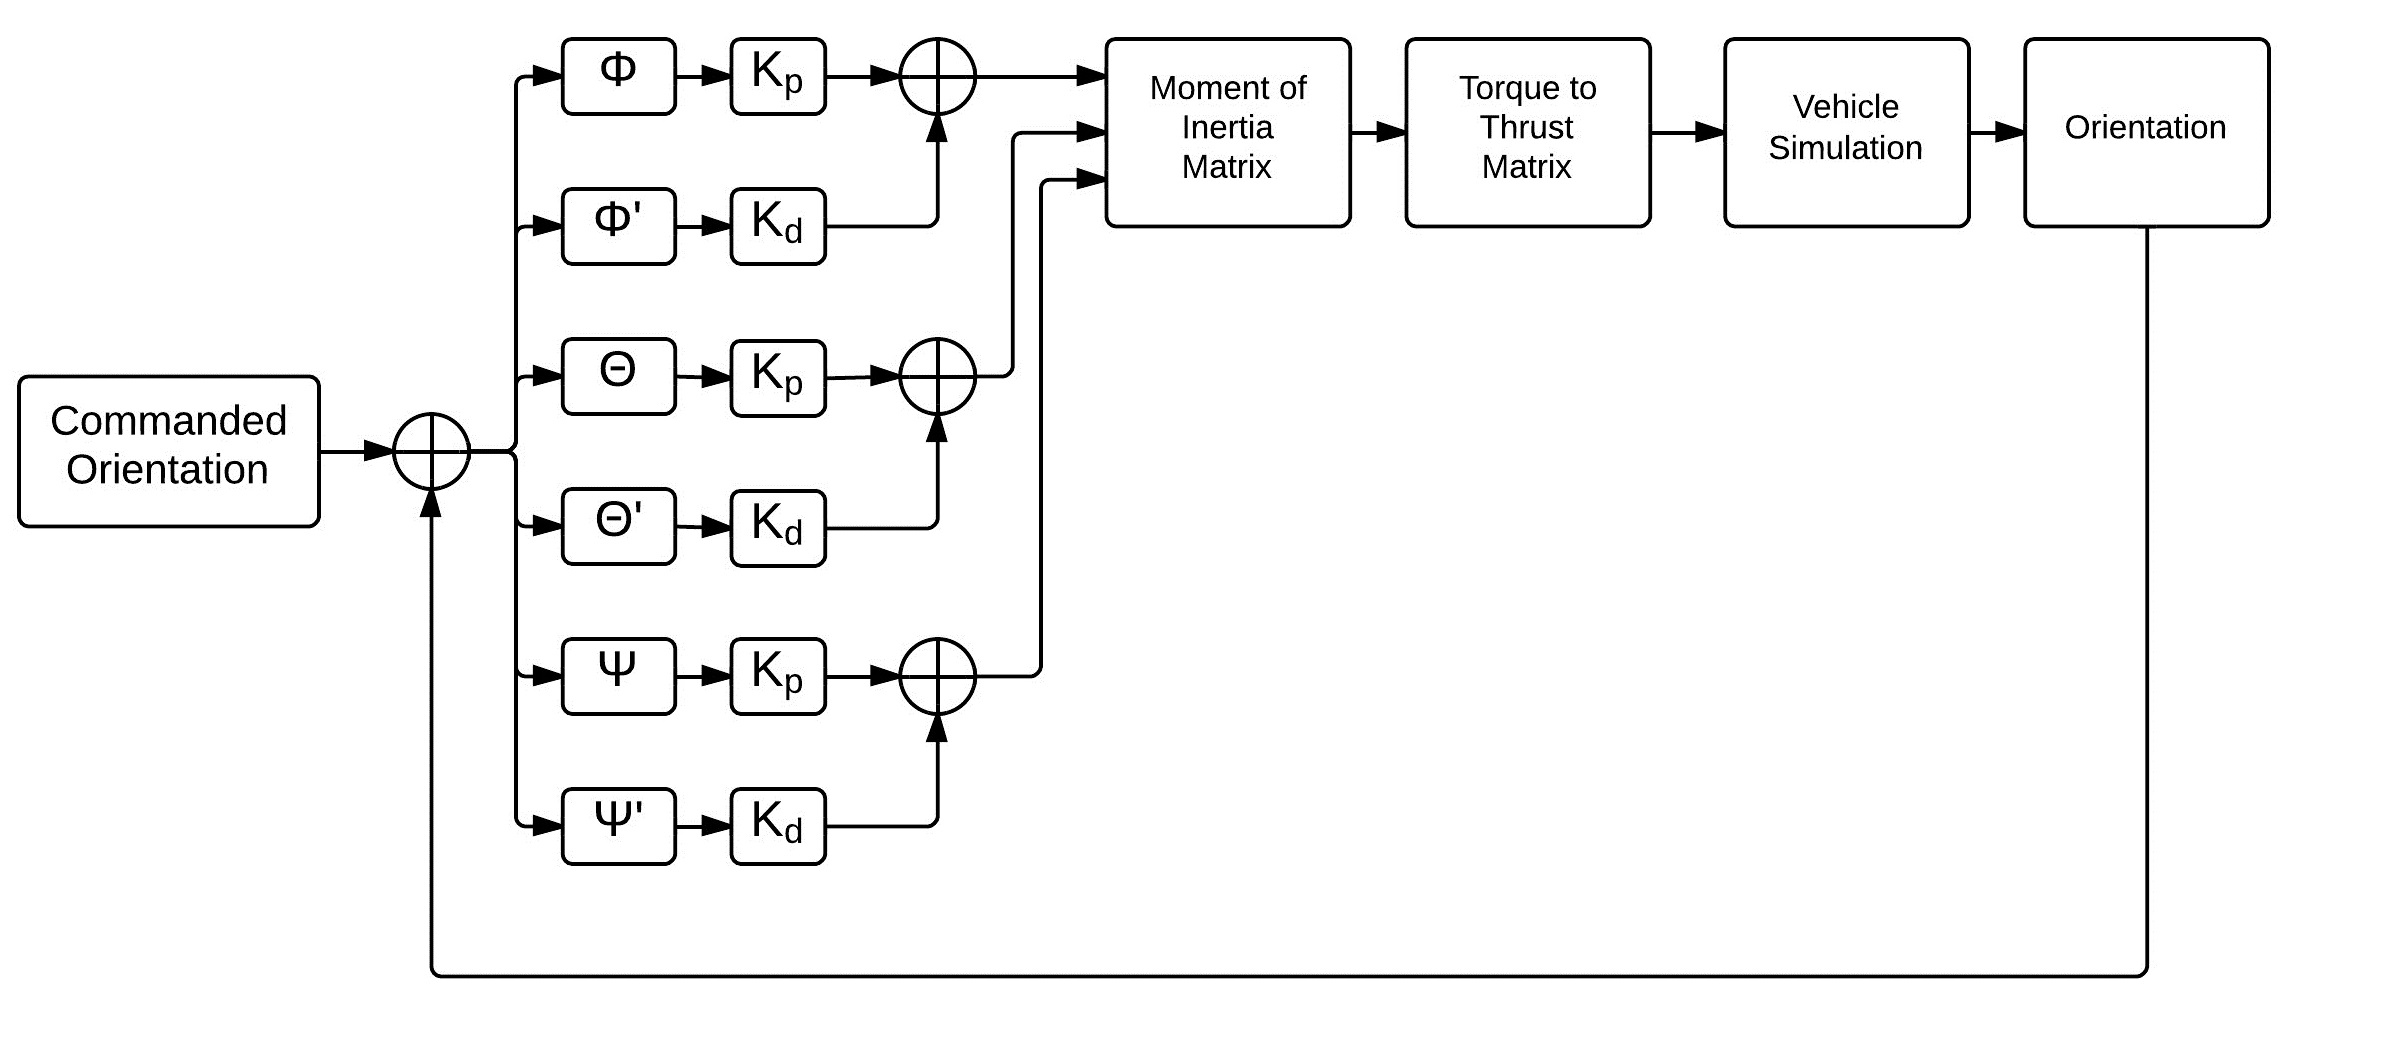
\includegraphics[width=1\textwidth]{Control}
\label{fig:control}
\end{figure}


\section{Results}

The controller successfully controls the attitude of the vehicle for random initial conditions that are bound by Euler angles of $\pm $1 radian. An example is shown in Figure ~\ref{fig:Response}.
\begin{figure}[H]
\caption{Attitude Control in Simulation.}
\center
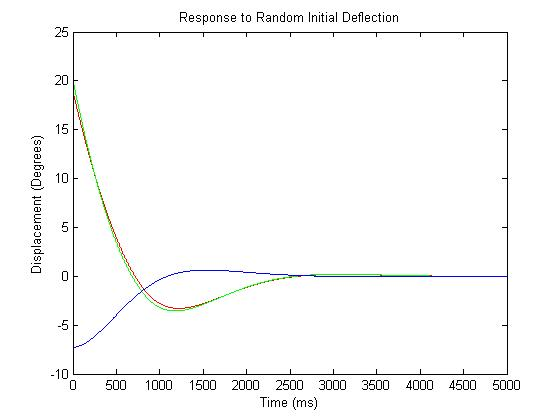
\includegraphics[width=0.9\textwidth]{Response}
\label{fig:Response}
\end{figure}
In the vehicle geometry analysis it was found that all configurations examined are highly invertible. In Figure ~\ref{fig:Invertibility} below the Invertibility of the thrust/momentum matrix is defined as the inverse of the condition number. Zero corresponds to a singular matrix and one corresponds to an involutory matrix (a matrix that is its own inverse). It can be seen from the figure that all matrices that were analyzed are sufficiently non-singular.
\begin{figure}[H]
\caption{Matrix Invertibility in Analyzed Configurations.}
\center
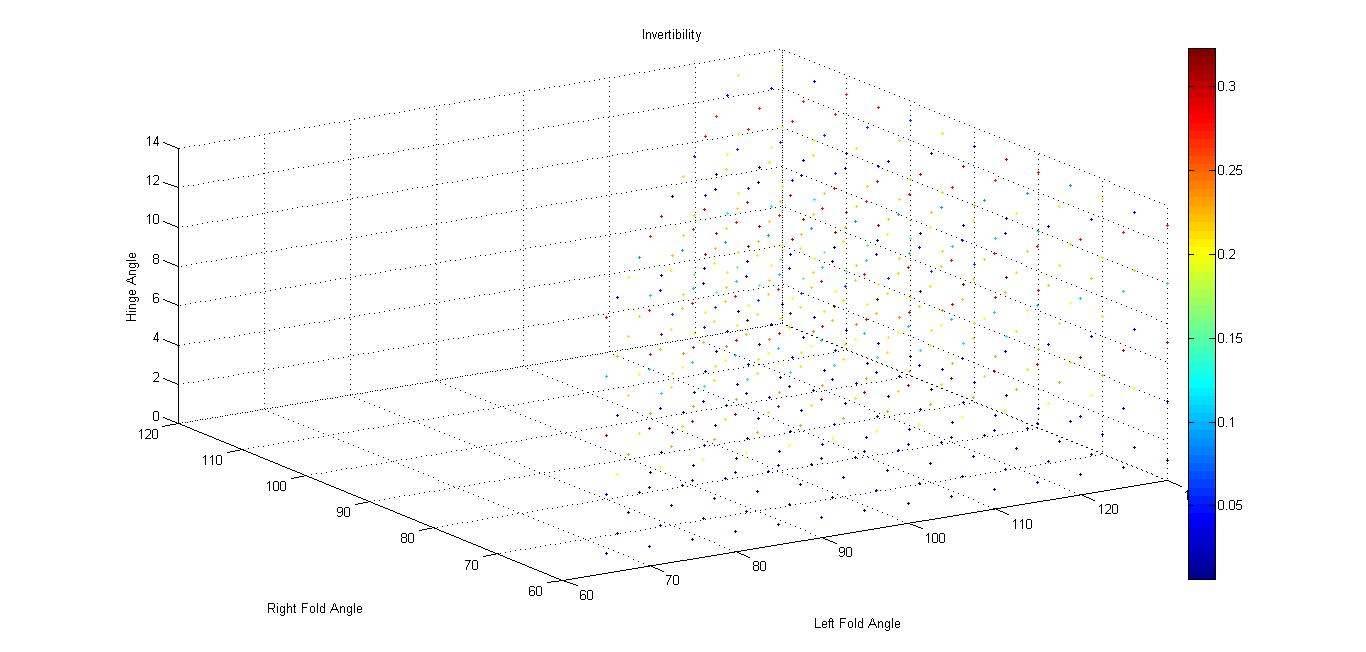
\includegraphics[width=1\textwidth]{Invertibility}
\label{fig:Invertibility}
\end{figure}
\section{Conclusion}

The simulation and analysis demonstrate the capability of the Pterodactyl design and serve as a means of validating controller designs. The folding design of the pterodactyl will merge the positive attributes of morphing vehicle capability and tailsitter configuration. As the design process continues, higher fidelity models will provide new insights into the system dynamics and validate the previous work.

\section{Future Work}

The work described in this paper represents the first step towards constructing the Pterodactyl UAS. Other major areas of work of note are vehicle guidance, forward flight control, mode transition control, autonomous landing, vehicle propulsion, and launch system design and construction.

\subsection{Forward Flight and Transition Control}

In its forward flight condition, the vehicle will be controlled using a standard GPS-based autopilot that can be tasked remotely. During transition to vertical flight, the vehicle will first perform a pull-up maneuver so that it is flying vertically. Once it establishes vertical flight, it will decelerate to hover and the wings will fold into place with the propulsors still running. A terminal descent is then initiated. A transitional flight controller must be built to handle this phase of flight as it is substantially different from both the forward flight and hover mode.

\subsection{Autonomous Landing}

Terminal descent guidance will be performed using a downward-looking IR camera system and a set of three IR beacons positioned at the landing site. The IR camera system will provide precise guidance corrections to the UAS during terminal descent, and will enable much higher landing accuracy than is currently achievable with GPS-based systems. This is necessary to meet the design goal of landing in such a small area as the mobile deployment platform described above.

\subsection{Vehicle Propulsion}
Propulsion may be provided either by gas-burning engines, electric motor/propeller combinations, or ducted fans. Trade studies involving propulsion technologies are currently being conducted. A wide range of options are currently feasible, and the ultimate design decisions will hinge on noise, endurance, and weight requirements. Simulation models of the Pterodactyl UAS will incorporate high-fidelity models of the propulsor systems and induced velocity flow over the aerodynamic body.

\subsection{Launch and Recovery System}
An important part of the development process will include design of the UAS launch and recovery system. The launcher will consist of a spring-loaded rail which can be fixed to a vehicle such as a pickup truck. A landing fixture will also be designed incorporating IR beacons for terminal guidance and latches that can be attached to the UAS once it has landed for storage and transportation.


\section*{Acknowledgments}

Thanks go to Trevor Bennett of Texas A\& M for his previous work on this concept.

\begin{thebibliography}{9}% maximum number of references (for label width)
\bibitem{Forshaw:2012}
Forshaw, J. L., and Lappas, V. J., “Transitional Control Architecture, Methodology, and Robustness for a Twin Helicopter 
Rotor Tailsitter,” \emph{AIAA Guidance, Navigation, and Control Conference,} 2012-4697, AIAA, Minneapolis, MN, 2012. 
 \bibitem{Barbarino:2011}
 Barbarino, S., Bilgen, O., Ajaj, R. M., Friswell, M. I., and Inman, D. J., "A Review of Morphing Aircraft," \emph{Journal of Intelligent Material Systems and Structures,} Vol. 22, 2011, pp. 823-851.
\bibitem{Wickenheiser:2008}
Wickenheiser, A., and Garcia, E., "Aerodynamic Modeling of Morphing Wings Using an Extended Lifting-Line Analysis", \emph{Journal of Aircraft}, Vol. 44, No. 1, 2007.
 \bibitem{Stone:2008}
 Stone, R.H., Anderson, P.,Hutchison, C., Tsai, A., Gibbens, P., and Wong, K.C., "Flight Testing of the T-Wing Tail-Sitter Unmanned Air Vehicle", \emph{Journal of Aircraft,} Vol. 45, No. 2, 2008
 \bibitem{Escareno:2007}
 Escareno, J., Stone, R., Sanchez, A., and Lozano, R., "Modeling and Control Strategy for the Transition of a Convertible Tail-Sitter UAV," \emph{European Control Conference 2007,} Kos, Greece, 2007.
 \bibitem{Matsumoto:2010}
Matsumoto, T., Kita, K., Suzuki, R., Oosedo, A., Go, K., Hoshino, Y., Konno, A., and Uchiyama, M., "A Hovering Control Strategy for a Tail-Sitter VTOL UAV that Increases Stability Against Large Disturbance," \emph{2010 IEEE International Conference on Robotics and Automation,} Anchorage, US, May 2010.

\end{thebibliography}

\end{document}

% - Release $Name:  $ -
